\section{Theorie}
\label{sec:Theorie}
Eine Brückenschaltung ist eine elektrische Schaltung, mit der in der Messtechnik diverse physikalische Größen über die Messung von
Widerständen bestimmt werden können. Zudem kann mit Brückenschaltungen durch die Nullmethode die Auflösung einer Messung erhöht werden.
Diese wird in den folgenden Abschnitten noch erläutert.

\subsection{Allgemeines zu Brückenschaltungen}
\label{sec:allg}
Eine Brückenschaltung besteht prizipell aus vier Widerständen. Diese sind so angeordnet, dass je zwei Widerstände in Reihe und
die in Reihe geschalteten Widerstände parallel geschaltet sind. Die Schaltung ist dabei an eine Speisespannung $U_S$ engeschlossen.
In Abbildung \ref{fig:allg} ist dieses Prinzip an einem Schaltbild verdeutlicht.

\begin{figure}[H]
    \centering
    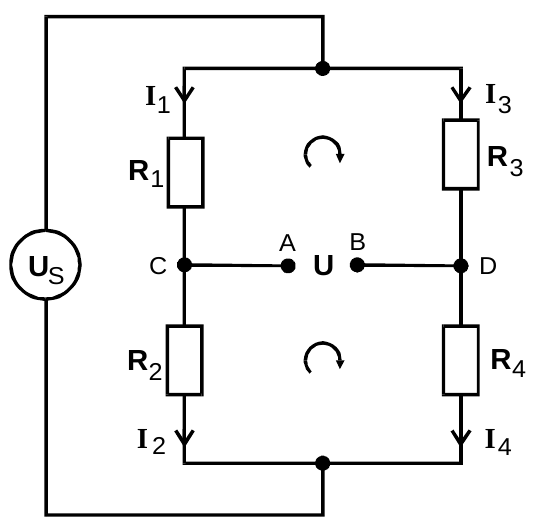
\includegraphics[scale=0.4]{pictures/1-allg.png}
    \caption{Prinzip einer Brückenschaltung. \cite{AP01}}
    \label{fig:allg}
\end{figure}
\noindent
Zwischen den eingezeichneten Punkten $A$ und $B$ entsteht eine Potentialdifferenz, die als Brückenspannung $U$ bezeichnet wird. Diese
kann über die Kirchhoff'schen Regeln hergeleitet werden. Die Kirchhoff'schen Regeln sind im Folgenden kurz beschrieben.

\begin{enumerate}
    \item\textbf{Knotenregel}
    \\\noindent
    Die Knotenregel besagt, dass die Summe aller eingehenden und ausgehenden Ströme in einem Knoten null ist, wobei eingehenden Strömen
    ein positives und ausgehenden ein negatives Vorzeichen zugeordnet wird. Die Knotenregel ist dabei äquivalent zu der Ladungserhaltung.
    Mathematisch ausgedrückt lautet sie
    \begin{equation}
        \sum_k I_k=0 \;.
        \label{eqn:kirchhoff1}
    \end{equation}

    \item\textbf{Maschenregel}
    \\\noindent
    Die Maschenregel besagt, dass die Summe aller Spannungen in einer Masche null ist. Eine Masche ist dabei ein geschlossener Stromkreis.
    Das Vorzeichen ist dabei abhängig von der Stromrichtung. So ist $U_K>0$ für einen mathematisch negativen Drehsinn und $I_K<0$ für einen
    positiven Drehsinn.Die Maschenregel ist äquivalent zu der Energieerhaltung. Sie wird beschrieben durch
    \begin{equation}
        \sum_k U_k=0 \;.
        \label{eqn:kirchhoff2}
    \end{equation}
\end{enumerate}
Durch Ausnutzen der Knotenregel wird schnell ersichtilich, dass in der Brückenschaltung \ref{fig:allg} $I_1=I_2$ und $I_3=I_4$ gilt.
Die Maschenregel liefert die beiden Gleichungen
\begin{align*}
    U &=-R_1I_1 + R_3I_3\\
    -U&=-R_2I_2 + R_4I_4 = -R_2I_1+R_4I_3 \;,
\end{align*}
welche durch Gleichsetzen zu
\begin{equation*}
    U=\frac{R_2R_3-R_1R_4}{R_3+R_4}I_1
\end{equation*}
führen. Mittels
\begin{equation*}
    U_S=I_1(R_1+R_2)
\end{equation*}
kann die Brückenspannung $U$ dann vollständig über die Widerstände und die Speisespannung $U_S$ ausgedrückt werden
\begin{equation}
    U=\frac{R_2R_3-R_1R_4}{(R_1+R_2)(R_3+R_4)}U_S\;.
    \label{eqn:brücke}
\end{equation}
Der Ausdruck \eqref{eqn:brücke} wird offensichtlich für
\begin{equation}
    R_1R_4=R_2R_3
    \label{eqn:abgleich}
\end{equation}
null. Für dieses Verhältnis an Widerständen wird von einer abgeglichenen Brücke gesprochen. Mit dieser kann ein unbekannter Widstand
ermittelt werden, indem mindestens einer der anderen drei so lange variiert wird, bis $U=0$ gilt.
\\\noindent
Die Brückenschaltung kann nun für Wechselströme auch auf komplexe Impedanzen $Z=X+jY$ erweitert werden, um neben Widerständen $R$ auch
Induktivitäten $L$ und Kondensatoren $C$ zuzulassen. Die verschiedenen Impedanzen sind dabei gegeben durch
\begin{align*}
    Z_C=-\frac{j}{\omega}C \qquad\quad
    Z_L=j\omega L          \qquad\quad
    Z_R=R \;,
\end{align*}
wobei $j$ ist imaginäre Einheit und $\omega$ die Kreisfrequenz ist. Die Abgleichbedingung ist analog zu jener mit reellen Widerständen
\eqref{eqn:abgleich} $Z_1Z_4=Z_2Z_3$. Für die Realteile folgt demnach
\begin{equation*}
    X_1X_4-Y_1Y_4=X_2X_3-Y_2Y_3
\end{equation*}
und für die Imaginärteile
\begin{equation*}
    X_1Y_4+X_4Y_1=X_2Y_3+X_3Y_2 \;.
\end{equation*}
Die Abgleichbedingung für Impedanzen besteht demnach aus zwei Gleichungen, welche den Betrag und die Phase beschreiben.

\subsection{Wheatstone'sche Brückenschaltung}
\label{sec:wheatstone}
\begin{figure}[H]
    \centering
    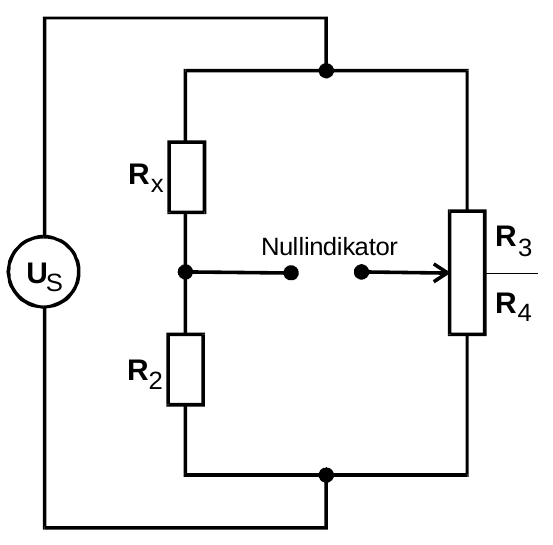
\includegraphics[scale=0.4]{pictures/2-wheatstone.png}
    \caption{Wheatstone'sche Brückenschaltung. \cite{AP01}}
    \label{fig:wheatstone}
\end{figure}
\noindent
Die Wheatstone'sche Brückenschaltung besitzt nur reelle Widerstände $R$ und kann somit für Gleich- und Wechselstrom verwendet werden.
Ziel ist es den unbekannten Widerstand $R_x$ zu bestimmen, indem die Abgleichbedingung \eqref{eqn:abgleich} ausgenutzt wird. Umstellen
ergibt
\begin{equation}
    R_x=R_2\frac{R_3}{R_4} \;.
    \label{eqn:wheatstone}
\end{equation}
Da es auf $R_3$ und $R_4$ im Speziellen nicht ankommt, sondern nur das Verhältnis relevant ist, sind diese beiden Widerstände wie in
Abbildung \ref{fig:wheatstone} zu erkennen als Potentiometer realisiert.

\subsection{Kapazitätsmessbrücke}
\label{sec:Cbrücke}
\begin{figure}[H]
    \centering
    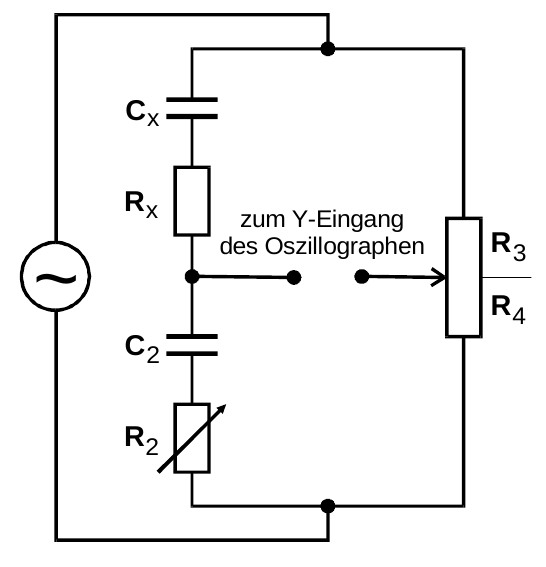
\includegraphics[scale=0.4]{pictures/3-C.png}
    \caption{Kapazitätsmessbrücke für reale Kondensatoren. \cite{AP01}}
    \label{fig:Cbrücke}
\end{figure}
\noindent
Bei der Kapazitätsbrücke (vgl. Abb. \ref{fig:Cbrücke}) wird ein unbekannter, realer Kondensator $C_x$ ausgemessen. Ein realer Kondensator
weist dabei im Gegensatz zu einem Idealen dielektrische Verluste auf, sodass er einen gewissen Widerstand $R$ besitzt. Die Impedanz
eines realen Kondensators ist also gegeben durch
\begin{equation}
    Z_{C,\text{real}}=R-\frac{j}{\omega}C \;.
\end{equation}
Da $Z_C$ sowohl Real- als auch Imaginärteil besitzt, kommen nun zwei Abgleichbedingungen zum tragen. Diese lauten
\begin{equation}
    R_x=R_2\frac{R_3}{R_4}
    \qquad\text{und}\qquad
    C_x=C_2\frac{R_4}{R_3} \;.
    \label{eqn:Cbrücke}
\end{equation}

\subsection{Induktivitätsmessbrücke}
\label{sec:Lbrücke}
\begin{figure}[H]
    \centering
    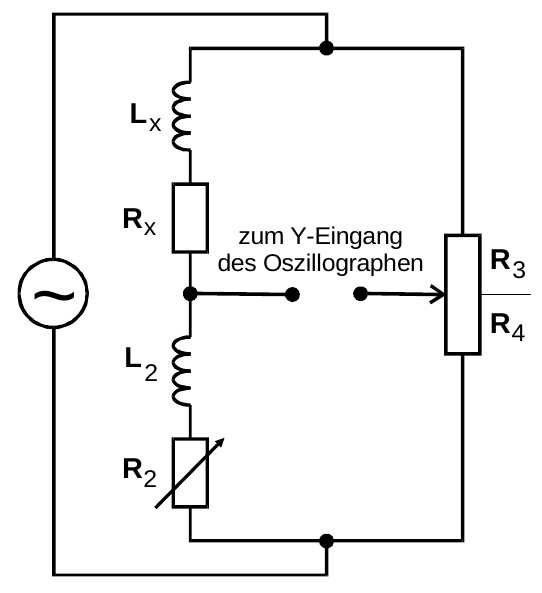
\includegraphics[scale=0.4]{pictures/4-L.png}
    \caption{Induktivitätsmessbrücke für reale Induktivitäten. \cite{AP01}}
    \label{fig:Lbrücke}
\end{figure}
\noindent
Die Induktivitätsmessbrücke (vgl. Abb. \ref{fig:Lbrücke}) ist prinzipell ähnlich zu der Kapazitätsbrücke \ref{sec:Cbrücke}, nur dass anstatt
eines realen Kondensators eine reale Induktivität $L_x$ ausgemessen wird. Eine reale Induktivität ist dabei analog zu dem realen Kondensator
verlustbehaftet, wobei diesmal magnetische Feldenergie in Wärme umgewandelt wird. Die reale Induktivität kann wieder über einen reeller
Widerstand und eine ideale Induktivität ausgedrückt werden, sodass sich für die Impedanz
\begin{equation*}
    Z_{L,\text{real}}=R+j\omega L
\end{equation*}
ergibt. Für die Abgleichbedingungen folgt
\begin{equation}
    R_x=R_2\frac{R_3}{R_4}
    \qquad\text{und}\qquad
    L_x=L_2\frac{R_3}{R_4} \;.
    \label{eqn:Lbrücke}
\end{equation}
Bei dieser Schaltung ist darauf zu achten, dass $L_2$ möglichst verlustfrei ist und dass der Wirktanteil möglichst allein durch $R_2$
realisiert ist. Da diese Forderungen gerade bei niedrigen Frequenzen nicht umsetztbar sind, werden für solche Messungen oft andere Schaltungen
wie die Maxwell-Brücke \ref{sec:maxwell} verwendet.

\subsection{Maxwell-Brücke}
\label{sec:maxwell}
\begin{figure}[H]
    \centering
    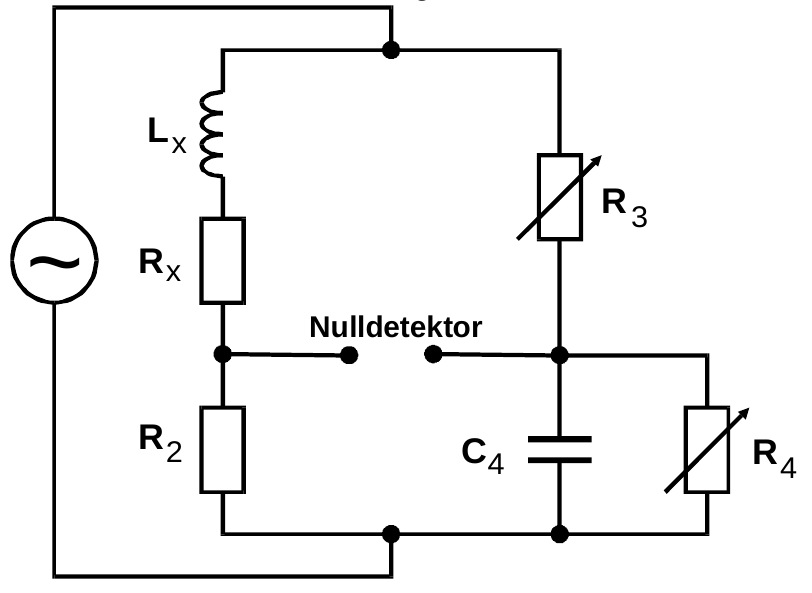
\includegraphics[scale=0.4]{pictures/5-maxwell.png}
    \caption{Maxwell-Brücke für reale Induktivitäten. \cite{AP01}}
    \label{fig:maxwell}
\end{figure}
\noindent
Auch mit der Maxwell-Brücke (vgl. Abb. \ref{fig:maxwell}) kann wie bei der Induktivitätsmessbrücke \ref{sec:Lbrücke} eine unbekannte,
reale Induktivität $L_x$ ausgemessen werden. Der Vorteil der Maxwellbrücke besteht jedoch darin, dass keine zweite Induktivität $L_2$
benötigt wird. Dafür ist ein Kondensator $C_4$ verbaut, welcher möglichst verlustarm sein sollte. Die regelbaren Widerstände $R_3$ und
$R_4$ stellen in dieser Schaltung die Abgleichelemente dar. Die Impedanzen sind der Form
\begin{equation}
    Z_1=R_x+j\omega L_x
    \qquad\text{und}\qquad
    Z_4=\frac{R_4-j\omega C_4R_4^2}{1+\omega^2C_4^2R_4^2} \;,
\end{equation}
womit sich die Abgleichbedingungen
\begin{equation}
    R_x=R_2\frac{R_3}{R_4}
    \qquad\text{und}\qquad
    L_x=R_2R_3C_4
    \label{eqn:maxwell}
\end{equation}
ergeben.

\subsection{Frequenzabhängigkeit der Abgleichbedingung}
\label{sec:frequenzabhängig}
Die in Abschnitt \ref{sec:allg} hergeleitete Abgleichbedingung \eqref{eqn:abgleich} ist unabhängig von der Frequenz der Speisespannung $U_S$.
Für große Frequenzen $\nu$ wird jedoch die Streukapazität in der Schaltung so groß, dass die beschreibenen Abgleichverfahren nicht mehr
möglich sind. Ist die Frequenz zu gering, kann der Abgleich erst nach einer längeren Einschwingphase erfolgen. Die optimale Frequenz liegt
dann vor, wenn der Wirkwiderstand $X$ die gleiche Größenordnung wie der Blindwiderstand $Y$ besitzt.
\\\noindent
Es gibt auch Schaltungen bei denen ein Abgleich nur bei diskreten Frequenzen möglich ist. Eine solche Schaltung wird im Folgenden
betrachtet.

\subsection{Wien-Robinson-Brücke}
\label{sec:wien-robinson}
\begin{figure}[H]
    \centering
    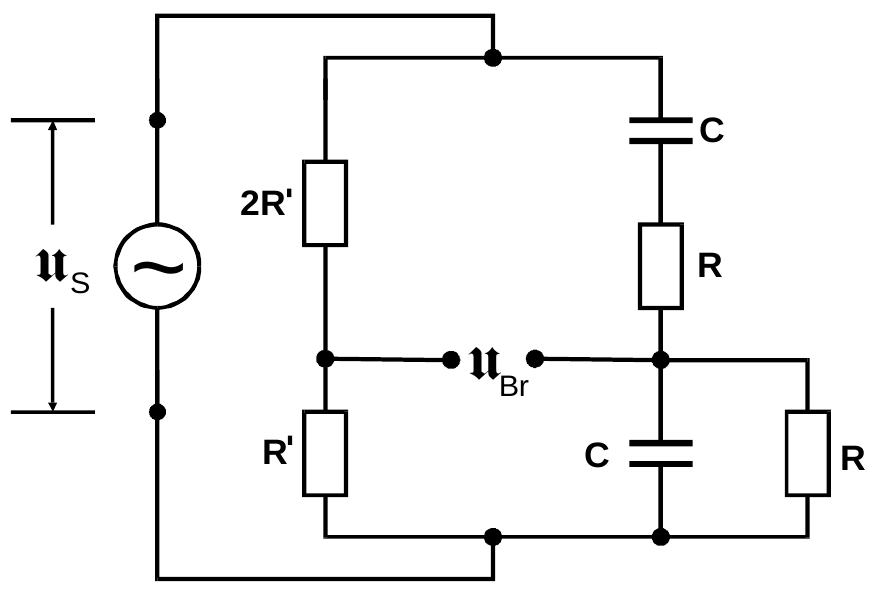
\includegraphics[scale=0.4]{pictures/6-wien-robinson.png}
    \caption{Wien-Robinson-Brücke. \cite{AP01}}
    \label{fig:wien-robinson}
\end{figure}
\noindent
Die Wien-Robinson-Brücke (vgl. Abb. \ref{fig:wien-robinson}) besitzt keine Abgleichelemente. Es ist desweiteren darauf zu achten, dass
$C$, $R$ und $R'$ möglichst genau bekannt sind und dass $C$ möglichst verlustfrei ist. Die Impedanzen in dieser Schaltung sind gegeben durch
\begin{equation*}
    Z_1=2R'\;,
    \qquad
    Z_2=R'\;,
    \qquad
    Z_3=\frac{j\omega CR+1}{j\omega C}\;,
    \qquad
    Z_4=\frac{R}{1+j\omega RC}\;.
\end{equation*}
Einsetzen in Gleichung \ref{eqn:brücke} liefert für die nun komplexe Brückenspannung $U_{Br}$
\begin{align*}
    U_{Br}&=\frac{\omega^2R^2C^2-1}{3(1-\omega^2R^2C^2)+9j\omega RC}U_S\\
    \Leftrightarrow
    \frac{U_{Br}}{U_S}&=\frac{\omega^2R^2C^2-1}{3(1-\omega^2R^2C^2)+9j\omega RC}\;.
\end{align*}
Die Bildung des Betragsquadrates ergibt
\begin{equation}
    \frac{U_{Br}}{U_S}=\frac{1}{9}\frac{\Omega^2-1}{(1-\Omega^2)^2+9\Omega^2}\;,
    \label{eqn:scheissformel}
\end{equation}
wobei $\Omega=\omega/\omega_0$ mit $\omega_0=1/LC$ ist. $\omega_0$ ist also genau die Nullstelle des Zählers. Die Schaltung entfernt demnach
die Frequenz $\omega_0$ aus einem kontinuierlichen Frequenzspektrum und kann somit als elektronischer Filter angesehen werden. Die um $\omega_0$
herum liegenden Frequenzen werden zudem noch stark abgeschwächt.
\\\noindent
Wird die Schaltung über einen Sinusgererator gespeißt, welcher gerade die Frequenz $\omega_0$ besitzt, kann mit der Wien-Robinson-Brücke
eine Untersuchung der Oberwellen, die durch den Generator erzeugt werden, durchführen. Das Verhältnis der Oberwellen $U_2$ bis $U_N$ zur
Grundwelle $U_1$ wird dabei als sogenannter Klirrfaktor definiert. Dieser ist gegeben durch
\begin{equation}
    k=\frac{\sqrt{\sum_{i=2}^N U_i^2}}{U_1}\;.
\end{equation}

%\subsection{TT-Brücke}
%\label{sec:TT}
%
%\begin{figure}[H]
%    \centering
%    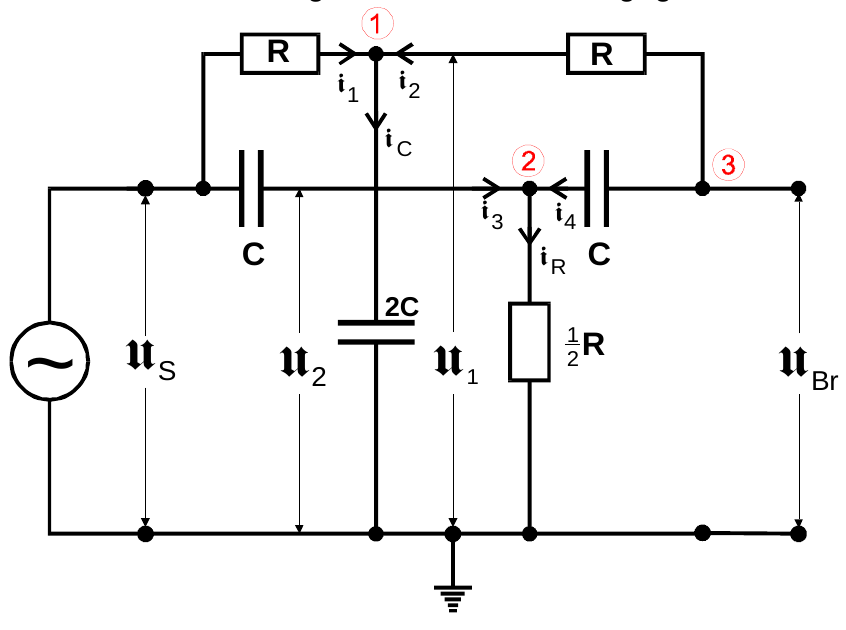
\includegraphics[scale=0.4]{pictures/7-TT.png}
%    \caption{TT-Brücke. \cite{AP01}}
%    \label{fig:TT}
%\end{figure}
